\chapter{Modulación AM}
\label{sec.ej3:am}

La modulación de amplitud convencional con portadora (AM o DSB) incorpora un nivel continuo de portadora
$E_c$ en conjunto con la señal de información $e_m(t)$, permitiendo que la envolvente de la señal de radiofrecuencia
reproduzca directamente la forma de onda de la señal modulante:
\begin{equation}
    v_{\mathrm{AM}}(t) = \left[E_c + e_m(t)\right] \cos(\omega_c t)
    \label{eq.am:temporal_gral}
\end{equation}
Para una señal modulante senoidal $e_m(t) = E_m \cos(\omega_m t)$, la expresión instantánea se reescribe como:
\begin{equation}
    v_{\mathrm{AM}}(t) = E_c \left[1 + m \cos(\omega_m t)\right] \cos(\omega_c t)
    \label{eq.am:temporal_indice}
\end{equation}
donde $m$ es el índice o factor de modulación, definido formalmente como el cociente entre la amplitud pico de la
modulante y la amplitud pico de la portadora:
\begin{equation}
    m = \frac{E_m}{E_c} = \frac{V_{\mathrm{max}} - V_{\mathrm{min}}}{V_{\mathrm{max}} + V_{\mathrm{min}}}
    \label{eq.am:indice_mod}
\end{equation}
siendo $V_{\mathrm{max}} = E_c (1 + m)$ y $V_{\mathrm{min}} = E_c (1 - m)$ los valores extremos de la envolvente.
Al expandir trigonométricamente la ecuación (\ref{eq.am:temporal_indice}), se obtiene la descomposición espectral:
\begin{equation}
    v_{\mathrm{AM}}(t) = E_c \cos(\omega_c t) + \frac{m E_c}{2} \cos\left((\omega_c - \omega_m)t\right) + \frac{m E_c}{2} \cos\left((\omega_c + \omega_m)t\right)
    \label{eq.am:espectro}
\end{equation}
A diferencia de DSB-SC, el espectro de AM conserva la componente de portadora en $\omega_c$ con una potencia fija
independiente de la modulación. El ancho de banda en RF es idéntico:
\begin{equation*}
    B_{\mathrm{AM}} = 2 f_m
\end{equation*}

\section{Condiciones Operativas y Señales de Excitación}
En la figura \ref{fig.am:kit} se aprecia el Kit N° 5 en su configuración para modulacion AM y demodulación. A diferencia
del montaje para DSB-SC, esta topología requiere alimentación dual con tensiones de $+12\V$ y $-8\V$, permitiendo fijar
la polarización de continua necesaria en los transistores del MC1496 para reinsertar la portadora en la señal de salida.
La placa incorpora los terminales de alimentación ($+12\V$, $-8\V$ y GND), el conector Mod In, Carrier In, el
potenciómetro de ajuste de portadora y las salidas Mod Out y Demo Out.

\begin{figure}[!ht]
    \centering
    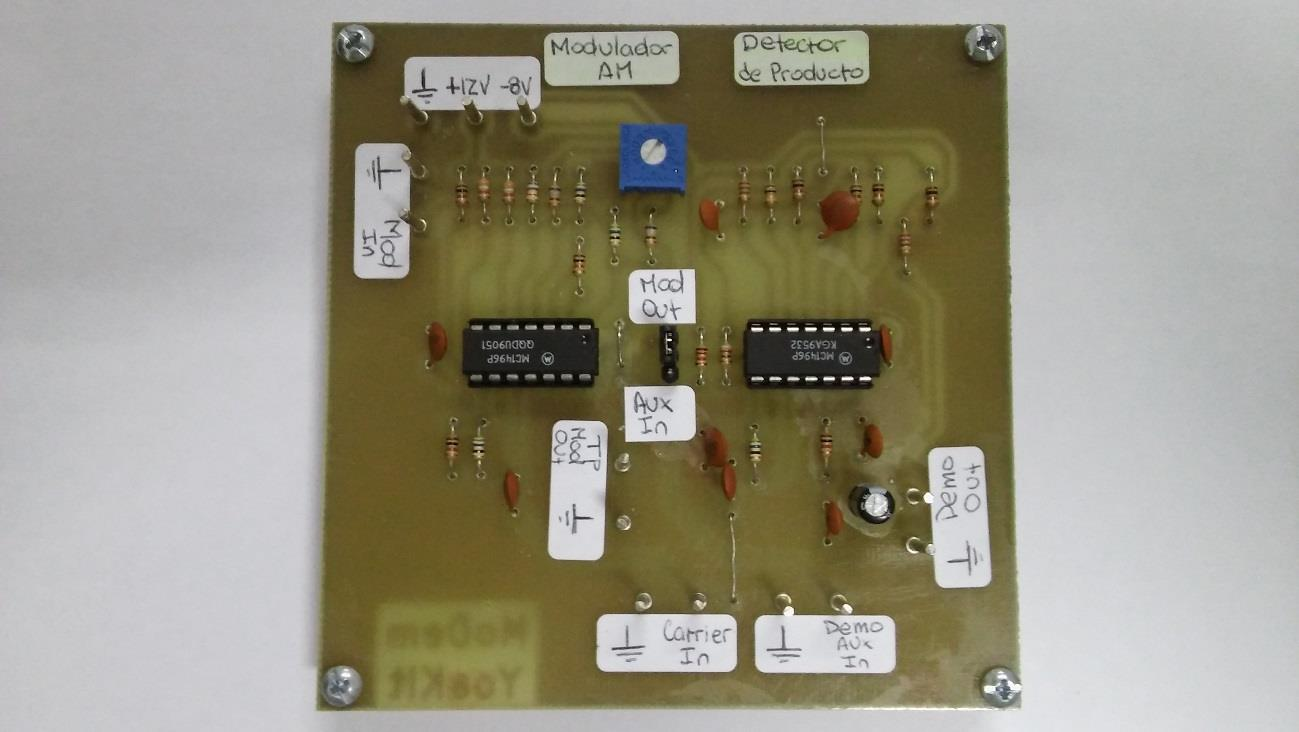
\includegraphics[width=0.68\textwidth]{pictures/kit_am.png}
    \caption{Placa de laboratorio del Kit N° 5.}
    \label{fig.am:kit}
\end{figure}

Para la configuración del kit en modo modulador AM, procedimos a energizar el módulo mediante una fuente de
alimentación dual ajustada en $+12\V$ y $-8\V$. Las señales de excitación se fijaron de acuerdo con la guía:
\begin{itemize}
    \item Portadora (Carrier In): señal senoidal de $f_c = 100\kHz$ con amplitud de $60\mVrms$.
    \item Modulante (Mod In): señal senoidal de $f_m = 10\kHz$ con amplitud de $300\mVrms$.
\end{itemize}

En la figura \ref{fig.am:entradas} se presentan las formas de onda capturadas en el osciloscopio digital.

\begin{figure}[!ht]
    \centering
    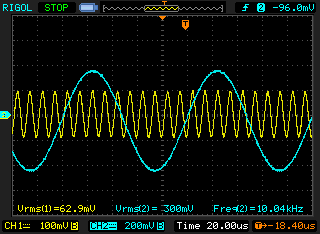
\includegraphics[width=0.68\textwidth]{images/NewFile12.png}
    \caption{Señales de excitación del modulador AM.}
    \label{fig.am:entradas}
\end{figure}

\section{Señal Modulada en Amplitud a la Salida}
Conectamos el Canal 2 a la salida modulada (Mod Out), manteniendo una base de tiempo de $10\,\unit{\micro\second}/\text{div}$
y una escala vertical de $100\mV/\text{div}$. La captura obtenida se expone en la figura \ref{fig.am:mod_out}.

\begin{figure}[H]
    \centering
    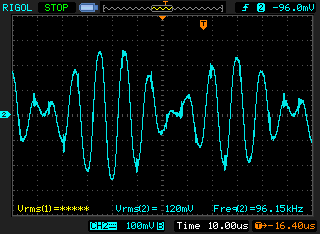
\includegraphics[width=0.68\textwidth]{images/NewFile13.png}
    \caption{Señal AM registrada a la salida Mod Out ($120\mVrms$, $100\mV/\text{div}$, $10\,\unit{\micro\second}/\text{div}$).}
    \label{fig.am:mod_out}
\end{figure}

\section{Análisis de los Regímenes de Modulación}
Variamos la amplitud de la señal modulante con el propósito de analizar experimentalmente los tres regímenes
característicos de modulación: submodulación ($m < 1$), modulación crítica o total ($m = 1$) y sobremodulación ($m > 1$).

\begin{figure}[!ht]
    \centering
    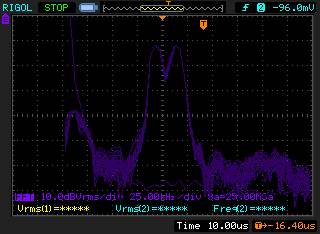
\includegraphics[width=0.6\textwidth]{images/NewFile14.png}
    \caption{Espectro en frecuencia (FFT).}
    \label{fig.am:fft_50}
\end{figure}

\begin{figure}[!ht]
    \centering
    \begin{subfigure}[t]{0.45\textwidth}
        \centering
        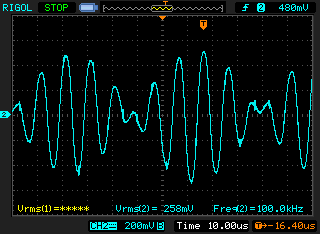
\includegraphics[width=\textwidth]{images/NewFile15.png}
        \caption{Dominio del tiempo.}
        \label{fig.am:mod_100_time}
    \end{subfigure}\hfill
    \begin{subfigure}[t]{0.45\textwidth}
        \centering
        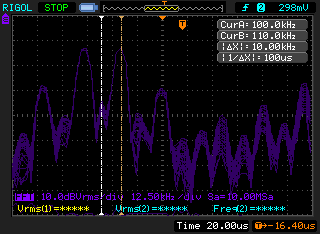
\includegraphics[width=\textwidth]{images/NewFile16.png}
        \caption{Dominio en frecuencia.}
        \label{fig.am:mod_100_fft}
    \end{subfigure}
    \caption{Comportamiento de la señal AM bajo modulación al $100\%$ ($m = 1{,}0$).}
    \label{fig.am:mod_100}
\end{figure}

\begin{figure}[H]
    \centering
    \begin{subfigure}[t]{0.45\textwidth}
        \centering
        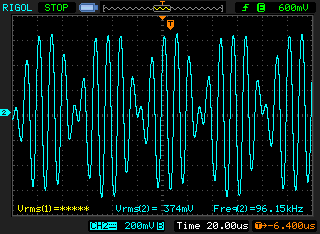
\includegraphics[width=\textwidth]{images/NewFile17.png}
        \caption{Dominio del tiempo.}
        \label{fig.am:sobremod_time}
    \end{subfigure}\hfill
    \begin{subfigure}[t]{0.45\textwidth}
        \centering
        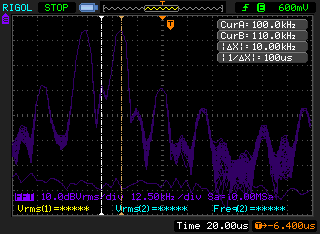
\includegraphics[width=\textwidth]{images/NewFile18.png}
        \caption{Dominio en frecuencia.}
        \label{fig.am:sobremod_fft}
    \end{subfigure}
    \caption{Comportamiento de la señal AM bajo modulación al $150\%$ ($m = 1{,}5$).}
    \label{fig.am:sobremod}
\end{figure}

\section{Efecto de la Variación en la Frecuencia Modulante}
Manteniendo fijo el nivel de modulación lineal, evaluamos la respuesta del modulador ante variaciones de la frecuencia
de banda base en dos puntos de ensayo: $f_m = 1\kHz$ y $f_m = 20\kHz$.

\begin{figure}[!ht]
    \centering
    \begin{subfigure}[t]{0.48\textwidth}
        \centering
        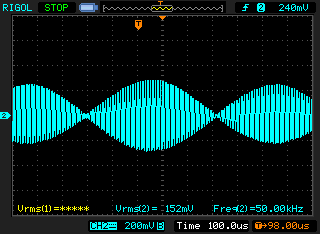
\includegraphics[width=\textwidth]{images/NewFile19.png}
        \caption{Dominio del tiempo.}
        \label{fig.am:freq_1k_time}
    \end{subfigure}\hfill
    \begin{subfigure}[t]{0.48\textwidth}
        \centering
        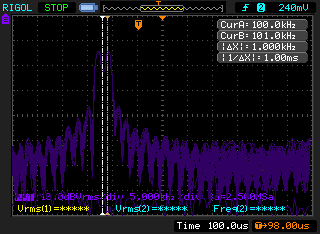
\includegraphics[width=\textwidth]{images/NewFile20.png}
        \caption{Dominio en frecuencia.}
        \label{fig.am:freq_1k_fft}
    \end{subfigure}
    \caption{Respuesta de modulación AM para modulante de baja frecuencia ($f_m = 1\kHz$).}
    \label{fig.am:freq_1k}
\end{figure}

\begin{figure}[H]
    \centering
    \begin{subfigure}[t]{0.48\textwidth}
        \centering
        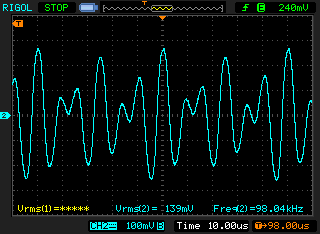
\includegraphics[width=\textwidth]{images/NewFile21.png}
        \caption{Dominio del tiempo.}
        \label{fig.am:freq_20k_time}
    \end{subfigure}\hfill
    \begin{subfigure}[t]{0.48\textwidth}
        \centering
        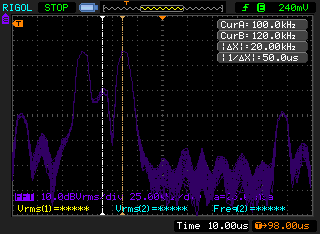
\includegraphics[width=\textwidth]{images/NewFile22.png}
        \caption{Dominio en frecuencia.}
        \label{fig.am:freq_20k_fft}
    \end{subfigure}
    \caption{Respuesta de modulación AM para modulante de alta frecuencia ($f_m = 20\kHz$).}
    \label{fig.am:freq_20k}
\end{figure}

\section{Demodulación y Etapa de Filtrado Activo}
Conectamos el osciloscopio en el conector Demo Out del kit para registrar la salida del detector de producto.
En la figura \ref{fig.am:demodulacion} se observa la señal recuperada, con una tensión eficaz de $V_{\mathrm{rms}} = 665\mV$.
La forma de onda principal reproduce el tono senoidal en baja frecuencia, pero presenta superpuesto un rizado
de alta frecuencia generado por la conmutación del producto y armónicos de portadora residual.

\begin{figure}[!ht]
    \centering
    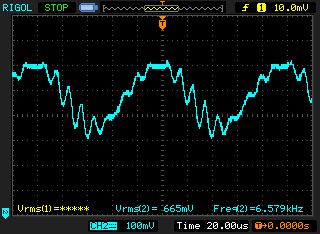
\includegraphics[width=0.68\textwidth]{images/NewFile23.png}
    \caption{Señal recuperada en la salida Demo Out ($665\mVrms$, $100\mV/\text{div}$, $20\,\unit{\micro\second}/\text{div}$).}
    \label{fig.am:demodulacion}
\end{figure}

\section{Control del Nivel de Portadora mediante Preset}
Finalmente, desconectamos la señal modulante en banda base y medimos la tensión de salida en Mod Out al actuar sobre
el preset de ajuste de portadora del kit, evaluando el rango dinámico de inserción de portadora en el MC1496:
\begin{itemize}
    \item Condición de mínima portadora (preset calibrado para máxima atenuación):
          en la figura \ref{fig.am:preset_min} se registró $V_{\mathrm{rms}} = 410\mV$ ($408\mVrms$ anotado en laboratorio),
          con una excursión entre cursores de $|\Delta Y| = 304\mV$.
    \item Condición de máxima portadora (preset ajustado a máxima reinserción):
          en la figura \ref{fig.am:preset_max} se registró $V_{\mathrm{rms}} = 805\mV$, con cursores en $|\Delta Y| = 76{,}0\mV$.
\end{itemize}

\begin{figure}[!ht]
    \centering
    \begin{subfigure}[t]{0.48\textwidth}
        \centering
        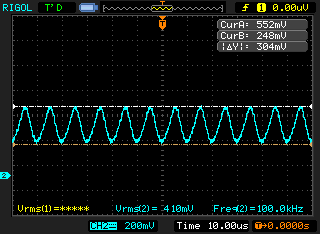
\includegraphics[width=\textwidth]{images/NewFile24.png}
        \caption{Nivel mínimo de portadora: $V_{\mathrm{rms}} = 408\mV$, $|\Delta Y| = 304\mV$.}
        \label{fig.am:preset_min}
    \end{subfigure}\hfill
    \begin{subfigure}[t]{0.48\textwidth}
        \centering
        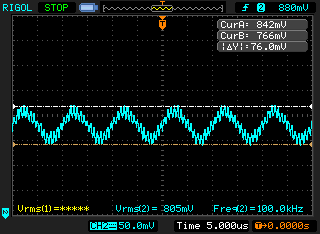
\includegraphics[width=\textwidth]{images/NewFile25.png}
        \caption{Nivel máximo de portadora: $V_{\mathrm{rms}} = 805\mV$, $|\Delta Y| = 76{,}0\mV$.}
        \label{fig.am:preset_max}
    \end{subfigure}
    \caption{Ajuste del nivel de portadora en salida sin señal de entrada mediante preset de polarización.}
    \label{fig.am:preset_portadora}
\end{figure}

El rango de variación logarítmico del nivel de portadora gobernado por el preset se cuantifica como:
\begin{equation}
    \Delta V_{\mathrm{c}} = 20 \log_{10}\left(\frac{V_{\mathrm{c,max}}}{V_{\mathrm{c,min}}}\right) = 20 \log_{10}\left(\frac{805\mV}{408\mV}\right) \approx 5{,}90\dB
    \label{eq.am:rango_preset}
\end{equation}
Esta variación de $5{,}90\dB$ demuestra experimentalmente la capacidad del MC1496 para operar como un modulador
multipropósito: introduciendo una corriente continua de desbalance se inyecta la portadora para transmitir en AM
estándar, mientras que anulando dicho desbalance se converge al régimen de portadora suprimida DSB-SC.
